\documentclass[11pt]{article}
\usepackage[utf8]{inputenc}
\usepackage[T1]{fontenc}
\usepackage{amsmath}
\usepackage{amsfonts}
\usepackage{amssymb}
\usepackage[version=4]{mhchem}
\usepackage{stmaryrd}
\usepackage{graphicx}
\usepackage[export]{adjustbox}
\graphicspath{ {./images/} }

\begin{document}
Commodity Risk Attributes

Many non-commodity-based investment strategies are exposed to large and often simultaneous event risk, such as losses from international tensions or financial turmoil (e.g., the global financial crisis of 2007-2008). Simply put, when a major global or economic crisis arises, long positions in most risky assets decline in value.

\section*{Four Favorable Characteristics of Commodities with Respect to Event Risks}
There are four characteristics of commodity investments that suggest that many major events actually enhance returns to investors with long positions in commodities.

First, most major global events cause increases in commodity prices due to anticipated decreases in commodity supplies or increases in demand. Events that may lead to unexpectedly reduced supply of one or more commodities include disrupted trade and disrupted production. Events such as trade wars, military wars, major weather events, and political instability can inhibit production and/or trade and drive up commodity prices. Trade disputes, wars, and political unrest tend to drive energy prices higher. Droughts, floods, and crop freezes tend to reduce the supply of agricultural products. Major labor unrest or global political instability can drive up the prices of and demand for both precious and industrial metals.

Second, commodity price increases due to events tend to be larger and more sudden than the price decreases resulting from events that lower commodity prices. These shocks to the commodity markets should provide long positions in commodities with positively skewed returns.

Third, many commodity shocks are likely to be uncorrelated with each other. For example, OPEC agreements to cut oil production should be uncorrelated with droughts in the agricultural regions around the world or with labor strikes affecting mining. The implication is that the commodity price changes due to major events should be relatively uncorrelated with each other and therefore somewhat diversifiable.

Fourth, shocks to the commodities markets are generally uncorrelated with shocks to the financial markets-or perhaps even negatively correlated. The reason is that most sudden large events have negative short-term implications to global production and trade. These shocks tend to reduce the supply of commodities, causing commodity prices to rise while simultaneously depressing equities and corporate bonds. For example, a shock such as a trade dispute or weather event may cause a sudden decrease in the supply of raw materials, which should have a positive impact on commodity prices but a negative impact on financial asset prices through its anticipated reduction in corporate profits.

\section*{Commodities as a Defensive Investment}
Fluctuations in aggregate global wealth are an unfortunate consequence of economic activity. When major declines in aggregate wealth occur (i.e., when major economic recessions or depressions occur), most major classes of investments tend to decline in response. A number of studies have examined the correlation of global equity markets during periods of market stress or decline. The conclusion is that equity markets around the world tend to be more highly correlated during periods of economic stress than during normal times. This means that in very bad times, when the benefits of diversification are most needed, equity markets throughout the world tend to decline at the same time, and global equity diversification fails to protect the investor. The major reason that traditional assets often do not provide downside risk protection is that almost all traditional assets react in similar fashion to major macroeconomic events. For example, a spike in oil prices is felt across almost all traditional asset classes.

Most traditional investments do not offer both protection from global turmoil and attractive returns. This is a major reason that investors are drawn to alternative investing. The greatest concern for most investors is downside risk. The ability to protect the value of an investment portfolio in hostile or turbulent markets is the key to the value of any macroeconomic diversification. Commodities may be especially useful at reducing downside risk.

\section*{Commodity Prices and Institutional Investing Demand}
One potential risk to long-only commodity investing is the impact of changes in institutional demand for long-only commodity positions. Historically, there was slow acceptance of commodity futures as a long-only investment by institutions such that institutional investment capital committed to commodity futures was considerably smaller than that invested with hedge funds. In the years prior to the global financial crisis of 2007-2008, large institutional investors sought greater diversification in their investment portfolios and established major long positions in commodities. This massive increase in the popularity of long-only commodity investing has been cited as a cause of large increases in the prices of commodities. Commodity prices collapsed during the financial crisis along with economic activity and prices in financial markets. While some attributed declining commodity prices to decisions by institutional investors to reduce long-only commodity exposures, there is evidence that there are many other factors at play. Notably, the prices of commodities without futures contracts or institutional investment also saw prices drop sharply during the global financial crisis (GFC).

Black ${ }^{1}$ K. Black, The Role of Institutional Investors in Rising Commodity Prices (2009), Journal of Investing 18 (no. 3): 21-26. seeks to downplay the role that institutional investors have played in commodity price volatility. Although it is plausible that their trading activity can influence commodity prices, other factors are likely more influential, especially in the energy markets, which are the largest sector in most commodity indices. Supply and demand for energy commodities, especially from biofuels, has a strong effect on prices. As many commodities worldwide are priced in US dollars, a strong US dollar likely contributes to weakness in commodity prices. Analysts also need to follow demand for commodities from China and other emerging markets, which can consume the majority of the world's commodity supplies despite having less than $20 \%$ of the value of global equity markets.

Irwin and Sanders ${ }^{2}$ S. H. Irwin and D. R. Sanders (2010), The Impact of Index and Swap Funds on Commodity Futures Markets: Preliminary Results, OECD Food, Agriculture and Fisheries Working Papers, No. 27 (2010), OECD Publishing. doi:10.1787/5kmd40wl1t5f-en. suggest that commodity index investing, with some caveats, may have decreased price volatility during the GFC. To the extent that commodity index investing provides more capital for taking the other side of hedging by commodity inventory holders, this means that more inventories can be held than otherwise would be the case. More inventories can help to reduce the chance of price spikes, which reduces price volatility.

Simply put: Short-term to medium-term long-only commodity returns may have volatility emanating from many sources, including commodity supply and demand, interest rates, inflation, trading activity, and currency markets.

\begin{center}
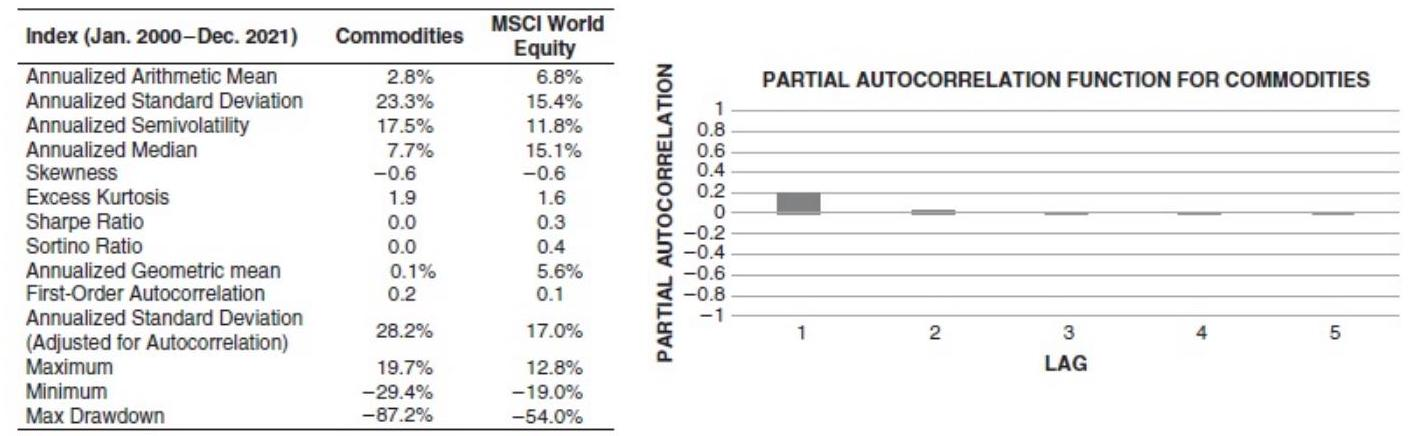
\includegraphics[max width=\textwidth]{2024_04_11_1a00330971bbdbb6beefg-3}
\end{center}

Histogram of Commodity Returns (Monthly) Jan. 2000-Dec. 2021

\begin{center}
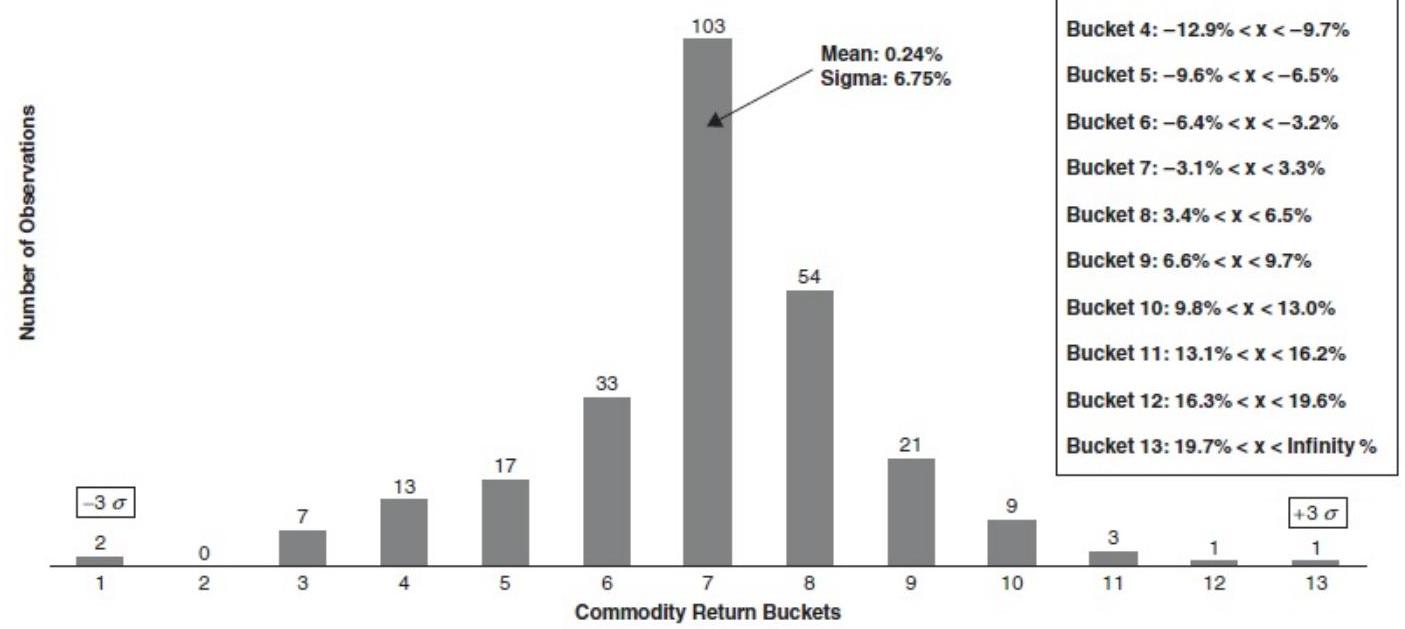
\includegraphics[max width=\textwidth]{2024_04_11_1a00330971bbdbb6beefg-3(1)}
\end{center}


\end{document}